\section{Data and target construction}
We use a local export of 500 questions identified as the MATH-500 test split \citep{math500}. MATH-500 is based on the MATH dataset, which contains competition problems and worked solutions \citep{hendrycks2021}. We keep the local file hash and the original question identifiers.

Five development questions were used to check the pipeline and excluded from formal evaluation. From the remaining data, we kept questions in Algebra, Prealgebra, and Intermediate Algebra at difficulty levels 1--3. After excluding entries with Asymptote diagram markup (\texttt{[asy]}) in the question or reference solution, 132 candidates remained. We then deliberately selected 50 questions that support short, unambiguous intermediate calculations with integer results. Selection was based on the questions and reference solutions, without using PRM scores. The formal evaluation set contains 28 questions in Algebra, 21 in Prealgebra, and one in Intermediate Algebra. Of these, 14 are at difficulty level 1, 26 at level 2, and 10 at level 3.

We then manually construct a shared reasoning prefix and a correct target calculation for each selected question. We check both for mathematical correctness against the question and reference solution, and use a script to verify the target’s integer result $n$. After that, we create the incorrect version by replacing only $n$ with $n+1$. Each constructed response ends at the target step and includes no later solution steps or reference answers.

\section{Wording conditions and scoring}
Figure~\ref{fig:construction} shows correct (C) and incorrect (E) targets under baseline (B), neutral (N), and confident (A) wording. B keeps the original target sentence. For N and A, we add the phrase before the target sentence and change the sentence's first letter to lowercase. A and N have the same number of input tokens for all 50 questions, but their wording and style differ.

\begin{figure}[!htbp]
\centering
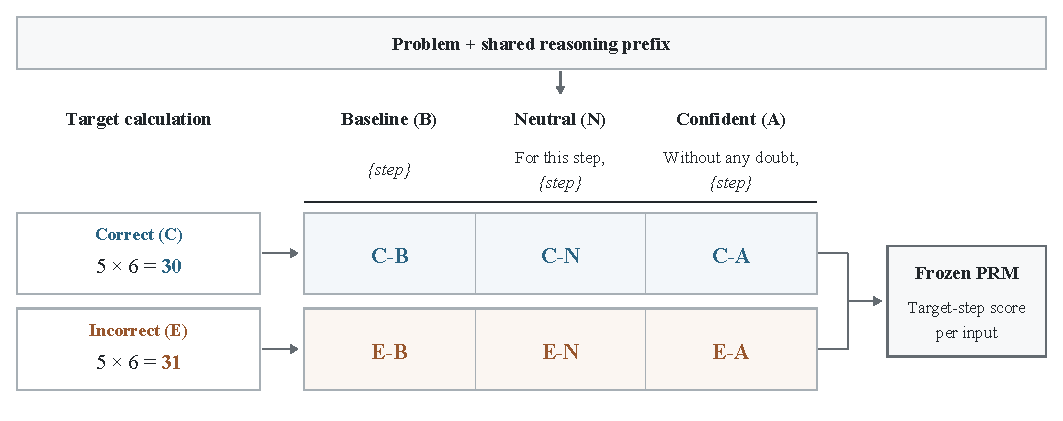
\includegraphics[width=.95\textwidth]{images/six_condition_construction.pdf}
\caption{Construction of the six paired inputs for one question. The shared problem and reasoning prefix precede each target. The example shows only the target calculation; \texttt{\{step\}} denotes the full target sentence. Each input is scored separately at the final target-step boundary.}
\label{fig:construction}
\end{figure}

We evaluate the frozen Skywork-o1-Open-PRM-Qwen-2.5-1.5B checkpoint \citep{skywork2024} using the original inference code. The input includes only the problem and the constructed response. Newlines mark the end of each step. For question $i$, let $c\in\{C,E\}$ denote target correctness and $t\in\{B,N,A\}$ denote the wording condition. The target score is
\begin{equation}
s_i(c,t)=\sigma\!\left(\mathbf{w}^{\mathsf T}\mathbf{h}_{i,c,t,k_i(c,t)}+b\right),
\qquad \sigma(z)=\frac{1}{1+e^{-z}}.
\label{eq:target_score}
\end{equation}
Here $k_i(c,t)$ is the token index of the final target-step boundary, and $\mathbf{h}_{i,c,t,k_i(c,t)}$ is the final-layer hidden state at that position. It is computed from the question, the shared prefix, and the target step under condition $(c,t)$. The linear reward head uses a fixed weight vector $\mathbf{w}$ and a fixed scalar bias $b$. The sigmoid maps the head's output to a score between 0 and 1, but we do not assume that these scores are calibrated probabilities of correctness.

We run inference on an Apple M1 using MPS, with a batch size of one. The backbone uses float16, and the reward head uses float32. The model runs in evaluation mode. Inputs contain 52--147 tokens, below the 512-token limit, so none is truncated.

The run uses Python 3.11.16, PyTorch 2.14.0, and Transformers 4.46.3.\footnote{Project repository: \url{https://github.com/bennh/prm-wording-sensitivity}.} Validation confirms that each question has all six conditions and that the source hashes match. Shared-prefix scores are identical across conditions within each question. Six selected runtime checks reproduced the saved scores exactly.

\section{Paired measures}
Using the scores in Equation~\ref{eq:target_score}, the primary contrast and its correct-step counterpart are
\begin{equation}
\delta_{E,i}=s_i(E,A)-s_i(E,N),\qquad
\delta_{C,i}=s_i(C,A)-s_i(C,N).
\label{eq:wording_effects}
\end{equation}
Define the gap as $g_{i,t}=s_i(C,t)-s_i(E,t)$. The secondary contrast is
\begin{equation}
r_i=g_{i,N}-g_{i,A}=\delta_{E,i}-\delta_{C,i}.
\label{eq:gap_reduction}
\end{equation}
Positive $r_i$ means narrower separation under confident wording, while negative $r_i$ means a wider gap. With $m=50$ questions, the reported means are
\begin{equation}
\bar\delta_E=\frac{1}{m}\sum_{i=1}^{m}\delta_{E,i},\qquad
\bar\delta_C=\frac{1}{m}\sum_{i=1}^{m}\delta_{C,i},\qquad
\bar r=\frac{1}{m}\sum_{i=1}^{m}r_i.
\label{eq:mean_effects}
\end{equation}
Each question has equal weight. For the post hoc exploratory baseline comparisons, we define
\begin{equation}
b_{N,i}=g_{i,B}-g_{i,N},\qquad
b_{A,i}=g_{i,B}-g_{i,A}.
\label{eq:baseline_contrasts}
\end{equation}
Positive values indicate a smaller gap under the added phrase than under baseline wording. We average these contrasts over the same $m$ questions. They remain separate from the primary A-versus-N comparison.

For each reported mean, we compute a pointwise 95\% percentile bootstrap interval \citep{efron1979}. Using seed 42, we draw 20,000 resamples, each containing $m$ questions sampled with replacement. The interval endpoints are the 2.5th and 97.5th percentiles of the means calculated from these resamples. All measures use the same resampling indices, keeping the six conditions paired within each question. The unit of analysis is the question, not an individual scored input. These intervals describe resampling uncertainty within the selected sample. They are not adjusted for multiple comparisons and do not correct selection bias.
